\chapter{Généralités sur les fonctions}
\section{Définitions}

\begin{definition}
  Étant donné un sous-ensemble $\mathcal{D}$ de $\mathbb{R}$, définir une \emph{fonction} de $\mathcal{D}$ dans $\mathbb{R}$, c'est associer à tout nombre $x$ de $\mathcal{D}$ un unique nombre $f(x)$ de $\mathbb{R}$.

  \begin{itemize}[$\bullet$]
    \item $\mathcal{D}$ est appelé \emph{ensemble de définition de $f$} ;
    \item $f(x)$ est \emph{l'image} de $x$ par $f$ ;
    \item $x$ est un \emph{antécédent} de $f(x)$ par $x$.
  \end{itemize}
\end{definition}

\begin{remarque}~
  \begin{itemize}
    \item Tout nombre $x$ de l'ensemble de définition de $f$ a une \emph{unique} image par $f$.
    \item Un nombre réel $a$ a zéro, un ou plusieurs antécédents par $f$.
  \end{itemize}
\end{remarque}

\begin{methode}~
  \begin{itemize}
    \item Pour trouver les antécédentes de $a$ par $f$, on résout l'équation $f(x)=a$.
    \item Pour déterminer l'image de $x$ par $f$, on calcule $f(x)$ en remplaçant $x$ par sa valeur dans la formule de $f$.
  \end{itemize}
\end{methode}

\section{Représentation graphique}

\subsection{Définitions}

\begin{definition}
  Dans le plan muni d'un repère, la \emph{courbe représentative} (ou \emph{représentation graphique}) de la fonction $f$ est l'ensemble $\mathcal{C}_f$ des points $(x, f(x))$, où $x$ décrit le domaine de définition de $f$.
\end{definition}

\begin{methode}
  Pour lire l'image de $x$ par $f$ :
  \begin{itemize}
    \item on repère $x$ sur l'axe des abscisses ;
    \item on trace la droite parallèle à l'axe des ordonnées d'abscisse $x$ ;
    \item on repère le point $M$, intersection de la courbe de $f$ et de la droite précédente ;
    \item on lit l'ordonnée de ce point $M$ : c'est l'image de $x$ par $f$.
  \end{itemize}
\end{methode}

\begin{methode}
  Pour lire les antécédents de $a$ par $f$ :
  \begin{itemize}
    \item on repère $a$ sur l'axe des ordonnées ;
    \item on trace la droite parallèle à l'axe des abscisses, d'ordonnée $a$ ;
    \item on repère les points d'intersection de la courbe de $f$ et cette droite ;
    \item on lit les abscisses de ces points d'intersection : ce sont les antécédents de $a$ par $f$.
  \end{itemize}
\end{methode}

\begin{remarque}
  Ces méthodes ne permettent que d'obtenir des valeurs approchées. Pour obtenir des valeurs exactes, le calcul de $f(x)$ ou la résolution algébrique de $f(x)=a$ sont nécessaires.
\end{remarque}

\subsection{Résolution graphique d'équation et d'inéquations}

\begin{propriete}
  \begin{itemize}
    \item Résoudre $f(x)=k$, c'est déterminer les antécédents de $k$ par $f$.
    \item Résoudre $f(x)=g(x)$, c'est déterminer les abscisses des points d'intersection de $f$ et $g$.
  \end{itemize}
\end{propriete}

\begin{propriete}
    Pour résoudre $f(x)\leq k$, on cherche les valeurs de $x$ dont l'image par $f$ est inférieure ou égale à $k$.

    Les solutions sont les abscisses des points de la courbe de $f$ dont l'ordonnée est inférieure ou égale à $k$.
\end{propriete}

\section{Variations}

\begin{definition}
  Un \emph{tableau de signes} permet de décrire les intervalles où une fonction est positive, et ceux où elle est négative.
\end{definition}

\subsection{(Dé)croissance}

\begin{definition}
  Soit $I$ un intervalle de $\mathbb R$, et $f$ une fonction définie sur $I$.
  \begin{itemize}
    \item $f$ est dite \emph{strictement   croissante} sur $I$ si pour tous
      réels $a$ et $b$ de $I$ tels que $a<b$, alors $f(a)<f(b)$.
    \item $f$ est dite \emph{strictement décroissante} sur $I$ si pour tous
      réels $a$ et $b$ de $I$ tels que $a<b$, alors $f(a)<f(b)$.
  \end{itemize}
\end{definition}

\begin{remarque}
  Graphiquement, la courbe représentative d'une fonction croissante
  « monte », tandis que celle d'une fonction décroissante « descend ».
\end{remarque}

\begin{exemple}
  Montrons que la fonction $f:x\mapsto 3x-1$ est croissante, et que la fonction
  $g:x\mapsto -2x+1$ est décroissante.
\end{exemple}

\subsection{Extrémums}

\begin{definition}
  Soit $I$ un intervalle de $\mathbb R$, $f$ une fonction définie sur $I$, et
  $a$ un élément de $I$.
  \begin{itemize}
    \item Si pour tout $x\in I$, $f(x)\leq f(a)$, on dit que $f(a)$ est le
      \emph{maximum} de $f$ sur $I$, atteint en $a$.
    \item Si pour tout $x\in I$, $f(x)\geq f(a)$, on dit que $f(a)$ est le
      \emph{minimum} de $f$ sur $I$, atteint en $a$.
    \item On appelle \emph{extremum} un minimum ou un maximum.
  \end{itemize}
\end{definition}

\begin{exemple}~
  \begin{multicols}{2}
    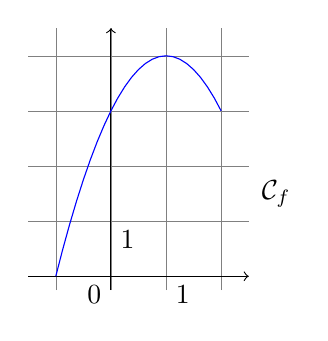
\begin{tikzpicture}[domain=-3:2.5, scale=0.7]
      \draw[very thin,color=gray,step=1] (-1.5,-0.25) grid (2.5,4.5);
      \draw[->] (-1.5,0) -- (2.5,0);
      \draw (1,0) node[below right] {1};
      \draw[->] (0,-0.25) -- (0,4.5);
      \draw (0,1) node[below right] {1};
      \draw (0,0) node[below left] {0};
      \draw[color=blue,domain=-1:2]
      plot (\x,{-(\x-3)*(\x+1)});
      \draw (3,1.5) node {${\cal C}_f$};
    \end{tikzpicture}

    La fonction $f$ (représentée ci-contre) est croissante sur $[-1;1]$, et décroissante sur $[1;2]$.

    Les extrémums de $f$ sont :
    \begin{itemize}
      \item $f(1)=4$, atteint en 1 ;
      \item $f(-1)=0$, atteint en -1.
    \end{itemize}

  \end{multicols}
\end{exemple}

\subsection{Tableau de variations}

\begin{definition}
  Un tableau de variations résume les informations connues à propos des variations d'une fonction.
\end{definition}
